\listfiles
\documentclass{article}

\usepackage[pdftex]{graphicx}
\usepackage{amsmath}
\usepackage{amssymb}

\usepackage[a4paper,margin=1in]{geometry}

\newcommand{\half}{\frac{1}{2}}

\title{The Bohr's Molecule}
\date{}

\begin{document}
\maketitle

\section{$\mathrm{H_2}$ molecule in equillibrium}

\subsection{$r/R$ and $\rho/R$}

Let $\theta$ be the angle subtended by the proton-electron line from the proton-proton line, i.e. the angle between the lines with length $R$ and $r$ respectively. Then, balancing the repulsive and attractive forces,

\begin{align*}
\frac{ke^2}{R^2} &= 2 \frac{ke^2}{r^2} \cos\theta
\end{align*}

noting that $\cos\theta = \frac{r}{2R}$,

\begin{align*}
\frac{1}{R^2} &= \frac{r/R}{r^2} \\
\frac{1}{R^2} &= \frac{r}{R} \\
R &= r
\end{align*}

hence the two protons and one electron form the vertices of an equilateral triangle. This makes sense as now the forces are of equal magnitude and all are $120^\circ$ from each other. Hence $\theta = \frac{\pi}{3}$ and

\begin{align*}
\frac{r}{R} = 1
\end{align*}

\begin{align*}
\frac{\rho}{R} &= \sin\frac{\pi}{3} \\
&= \frac{\sqrt 3}{2}
\end{align*}

\subsection{$E_p$}

Let $E_{pp}$ be the electric potential energy between a pair of protons in the configuration, $E_{pe}$ be the electric potential energy between a proton and an electron, and $E_{ee}$ be that between two electrons. Then

\begin{align*}
E_{pp} &= \frac{ke^2}{R} \\
E_{pe} &= -\frac{ke^2}{r} \\
&= -\frac{ke^2}{R} \\
E_{ee} &= \frac{ke^2}{2\rho} \\
&= \frac{ke^2}{2R} \frac{2}{\sqrt 3} \\
&= \frac{ke^2}{R} \frac{\sqrt 3}{3}
\end{align*}

since there is one pair of protons, one of electrons and 4 proton-electron pairs,

\begin{align*}
E_p &= E_{pp} + E_{ee} + 4 E_{pe} \\
&= \frac{ke^2}{R} \left(\frac{\sqrt 3}{3} - 3\right)
\end{align*}

\subsection{$E_k/E_p$}

Let $F_c$ be the centripetal force pulling the electron in. Then

\begin{align*}
F_c &= 2 \frac{ke^2}{R^2} \cos\frac{\pi}{6} - \frac{ke^2}{(2\rho)^2} \\
&= \frac{ke^2}{R^2}\left(\sqrt{3} - \frac{1}{3}\right)
\end{align*}

Also,

\begin{align*}
F_c &= \frac{m_e v^2}{\rho} \\
&= \frac{m_e v^2}{R} \frac{2\sqrt 3}{3}
\end{align*}

So

\begin{align*}
\frac{m_e v^2}{R} \frac{2\sqrt 3}{3} &= \frac{ke^2}{R^2}\left(\sqrt{3} - \frac{1}{3}\right) \\
m_e v^2 &= \frac{ke^2}{R}\left(\sqrt{3} - \frac{1}{3}\right) \frac{\sqrt 3}{2} \\
&= \frac{ke^2}{R}\left(\frac{9 - \sqrt 3}{6}\right)
\end{align*}

Since there are two electrons, $E_k = 2 (\frac{1}{2} m_e v^2) = m_e v^2$

\begin{align*}
E_k = \frac{ke^2}{R}\left(\frac{9 - \sqrt 3}{6}\right)
\end{align*}

So

\begin{align*}
\frac{E_k}{E_p} &= \frac{\frac{ke^2}{R}\left(\frac{9 - \sqrt 3}{6}\right)}{\frac{ke^2}{R} \left(\frac{\sqrt 3}{3} - 3\right)} \\
&= -\frac{1}{2}
\end{align*}

\subsection{$R_0$}

Now

\begin{align*}
m_e v^2 = \frac{ke^2}{R}\left(\frac{9 - \sqrt 3}{6}\right)
\end{align*}

and so

\begin{align*}
v = \sqrt{\frac{ke^2}{m_eR}\left(\frac{9 - \sqrt 3}{6}\right)}
\end{align*}

the momentum $p$ is

\begin{align*}
p &= m_e v \\
&= \sqrt{\frac{m_eke^2}{R}\left(\frac{9 - \sqrt 3}{6}\right)}
\end{align*}

since the momentum of the electron about the center of the molecule is perpenducal to the radial vector to the electron, $L = \rho p = Rp \frac{\sqrt{3}}{2}$ and

\begin{align*}
L &= \frac{\sqrt{3}}{2} R p \\
&= \frac{\sqrt{3}}{2} \sqrt{m_eRke^2\left(\frac{9 - \sqrt 3}{6}\right)} \\
&= \sqrt{m_eRke^2\left(\frac{9 - \sqrt 3}{8}\right)} \\
&= n\hbar
\end{align*}

$R$ will be minimized when $n$ is the smallest, which occurs when $n=1$

\begin{align*}
\sqrt{m_eR_0ke^2\left(\frac{9 - \sqrt 3}{8}\right)} &= \hbar \\
R_0 &= \frac{\hbar^2}{km_e e^2} \left(\frac{8}{9 - \sqrt 3}\right) \\
&= 5.82478 \times 10^{-11}\ m
\end{align*}

\subsection{$E_b$}

The total energy of the molecule is

\begin{align*}
E &= E_k + E_p \\
&= \frac{ke^2}{R_0} \left(\frac{3}{2} - \frac{\sqrt 3}{6} + \frac{\sqrt 3}{3} - 3\right) \\
&= -29.946\ eV
\end{align*}

wheares the energy of the hydrogen atom is $E_I$. Hence the binding energy, which is the difference between the energy of a $\mathrm{H_2}$ molecule and two $H$ atoms, is

\begin{align*}
E_b &= -2 E_I - E \\
&= 29.946\ eV - 2(13.606\ eV) \\
&= 2.73\ eV
\end{align*}

\section{Vibrating $\mathrm{H_2}$ molecule}

\subsection{Morse potential}

We sketch the morse potential with $D=R_0=\alpha=1$.

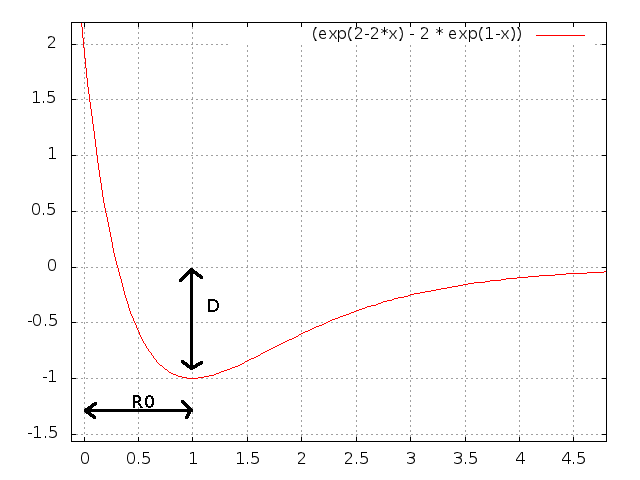
\includegraphics[width=\textwidth]{morse.png}

Clearly the potential reaches a minimum at $R = R_0$ where it has the minimum value of $D$. We can see this more clearly by writing $E(R) = (1 - e^{1-x})^2 - 1$. There is a horizontal asymptote at $E = 0$. $\alpha$ seems to control the `width' of the dip.

\subsection{$D$ and $E_b$}

\begin{align*}
\mathrm{When}\ R = R_0&, E = -D \\
\mathrm{As}\ R \rightarrow \infty&, E \rightarrow 0
\end{align*}

Hence the bonding energy $E_b = D$.

\subsection{Linear frequency of vibration}

Let $F(R)$ be the force exerted on the electron. Then

\begin{align*}
F(R) &= -\frac{dE}{dR} \\
&= \frac{2\alpha D}{R_0}\left(e^{2\alpha(1-R/R_0)} - e^{\alpha(1 - R/R_0)}\right)
\end{align*}

as expected, $F(R_0) = 0$, so $R_0$ is an equilibrium position and the system will oscillate around it. Let $r$ be a small increase in $R$; then

\begin{align*}
F(R_0 + r) &= \frac{dF}{dR}\Big|_{R_0} r
\end{align*}

so

\begin{align*}
\frac{dF}{dR}\Big|_{R_0} &= -\frac{2\alpha^2D}{R_0^2} \left(2e^{2\alpha(1-R/R_0)} - e^{\alpha(1-R/R_0)}\right) \Big|_{R_0} \\
&= -\frac{2\alpha^2D}{R_0^2}
\end{align*}

Let the acceleration be $\ddot{r}$

\begin{align*}
\ddot{r} &= \frac{F}{m_p} = -\frac{2\alpha^2D}{m_pR_0^2} r
\end{align*}

Let $\omega$ be the angular frequency; then 

\begin{align*}
\omega &= \sqrt\frac{2\alpha^2D}{m_pR_0^2} \\
&= \frac{\alpha}{R_0}\sqrt\frac{2E_b}{m_p}
\end{align*}

\begin{align*}
v_{vib} &= \frac{\omega}{2\pi} \\
&= \frac{\alpha}{2\pi R_0}\sqrt\frac{2E_b}{m_p}
\end{align*}

\subsection{$\alpha$ constant}

The energy of a photon is $hc/\lambda$; hence the photon lost in the Raman process is

\begin{align*}
\frac{hc}{\lambda_i} - \frac{hc}{\lambda_s} = h v_{vib}
\end{align*}

so

\begin{align*}
v_{vib} &= c\left(\frac{1}{514\mathrm{\ nm}} - \frac{1}{664\mathrm{\ nm}}\right) \\
&= 1.32 \times 10^{14}\mathrm{\ s^{-1}}
\end{align*}

and the energy lost was $0.54$ eV.

\begin{align*}
\alpha &= 2\pi R_0 v_{vib} \sqrt\frac{m_p}{2E_b} \\
&= 2.11
\end{align*}

\subsection{Minimum amplitude}

We approximate E by a taylor series

\begin{align*}
E(R_0 + r) = E(R_0) + \frac{1}{2} \frac{d^2E}{dR^2}\Big|_{R_0} r^2 + O(r^3)
\end{align*}

and

\begin{align*}
\frac{1}{2} \frac{d^2E}{dR^2}\Big|_{R_0} &= \frac{\alpha^2D}{R_0^2} \\
&= 3.58 \times 10^{21}\mathrm{\ eV\ m}^{-2}
\end{align*}

We know that $E(R_0 + A_{min}) = 0.54$ eV; hence

\begin{align*}
A_{min} &= \sqrt\frac{0.54\mathrm{\ eV}}{3.58 \times 10^{21}\mathrm{\ eV\ m}^{-2}}\\
&= 1.23 \times 10^{-11} \mathrm{\ m}
\end{align*}

\end{document}
